\documentclass[a4paper, 11pt, oneside]{article}
% Load encoding definitions (after font package)
\usepackage[T1]{fontenc}
\usepackage[default]{frcursive}
\usepackage{textalpha}
\usepackage{graphicx}
\usepackage{float}
\graphicspath{ {./} }
\usepackage[figurename=]{caption}
\usepackage{listings}
\usepackage{subcaption}
\lstset{basicstyle=\ttfamily}

% Babel package:
\usepackage{babel}


\usepackage[dvipsnames]{xcolor}
\usepackage{eso-pic,graphicx}
\usepackage[top=105mm, bottom=60mm, outer=55mm, inner=55mm]{geometry}
\setlength{\columnsep}{70pt}
\color{Black}
\AddToShipoutPictureBG{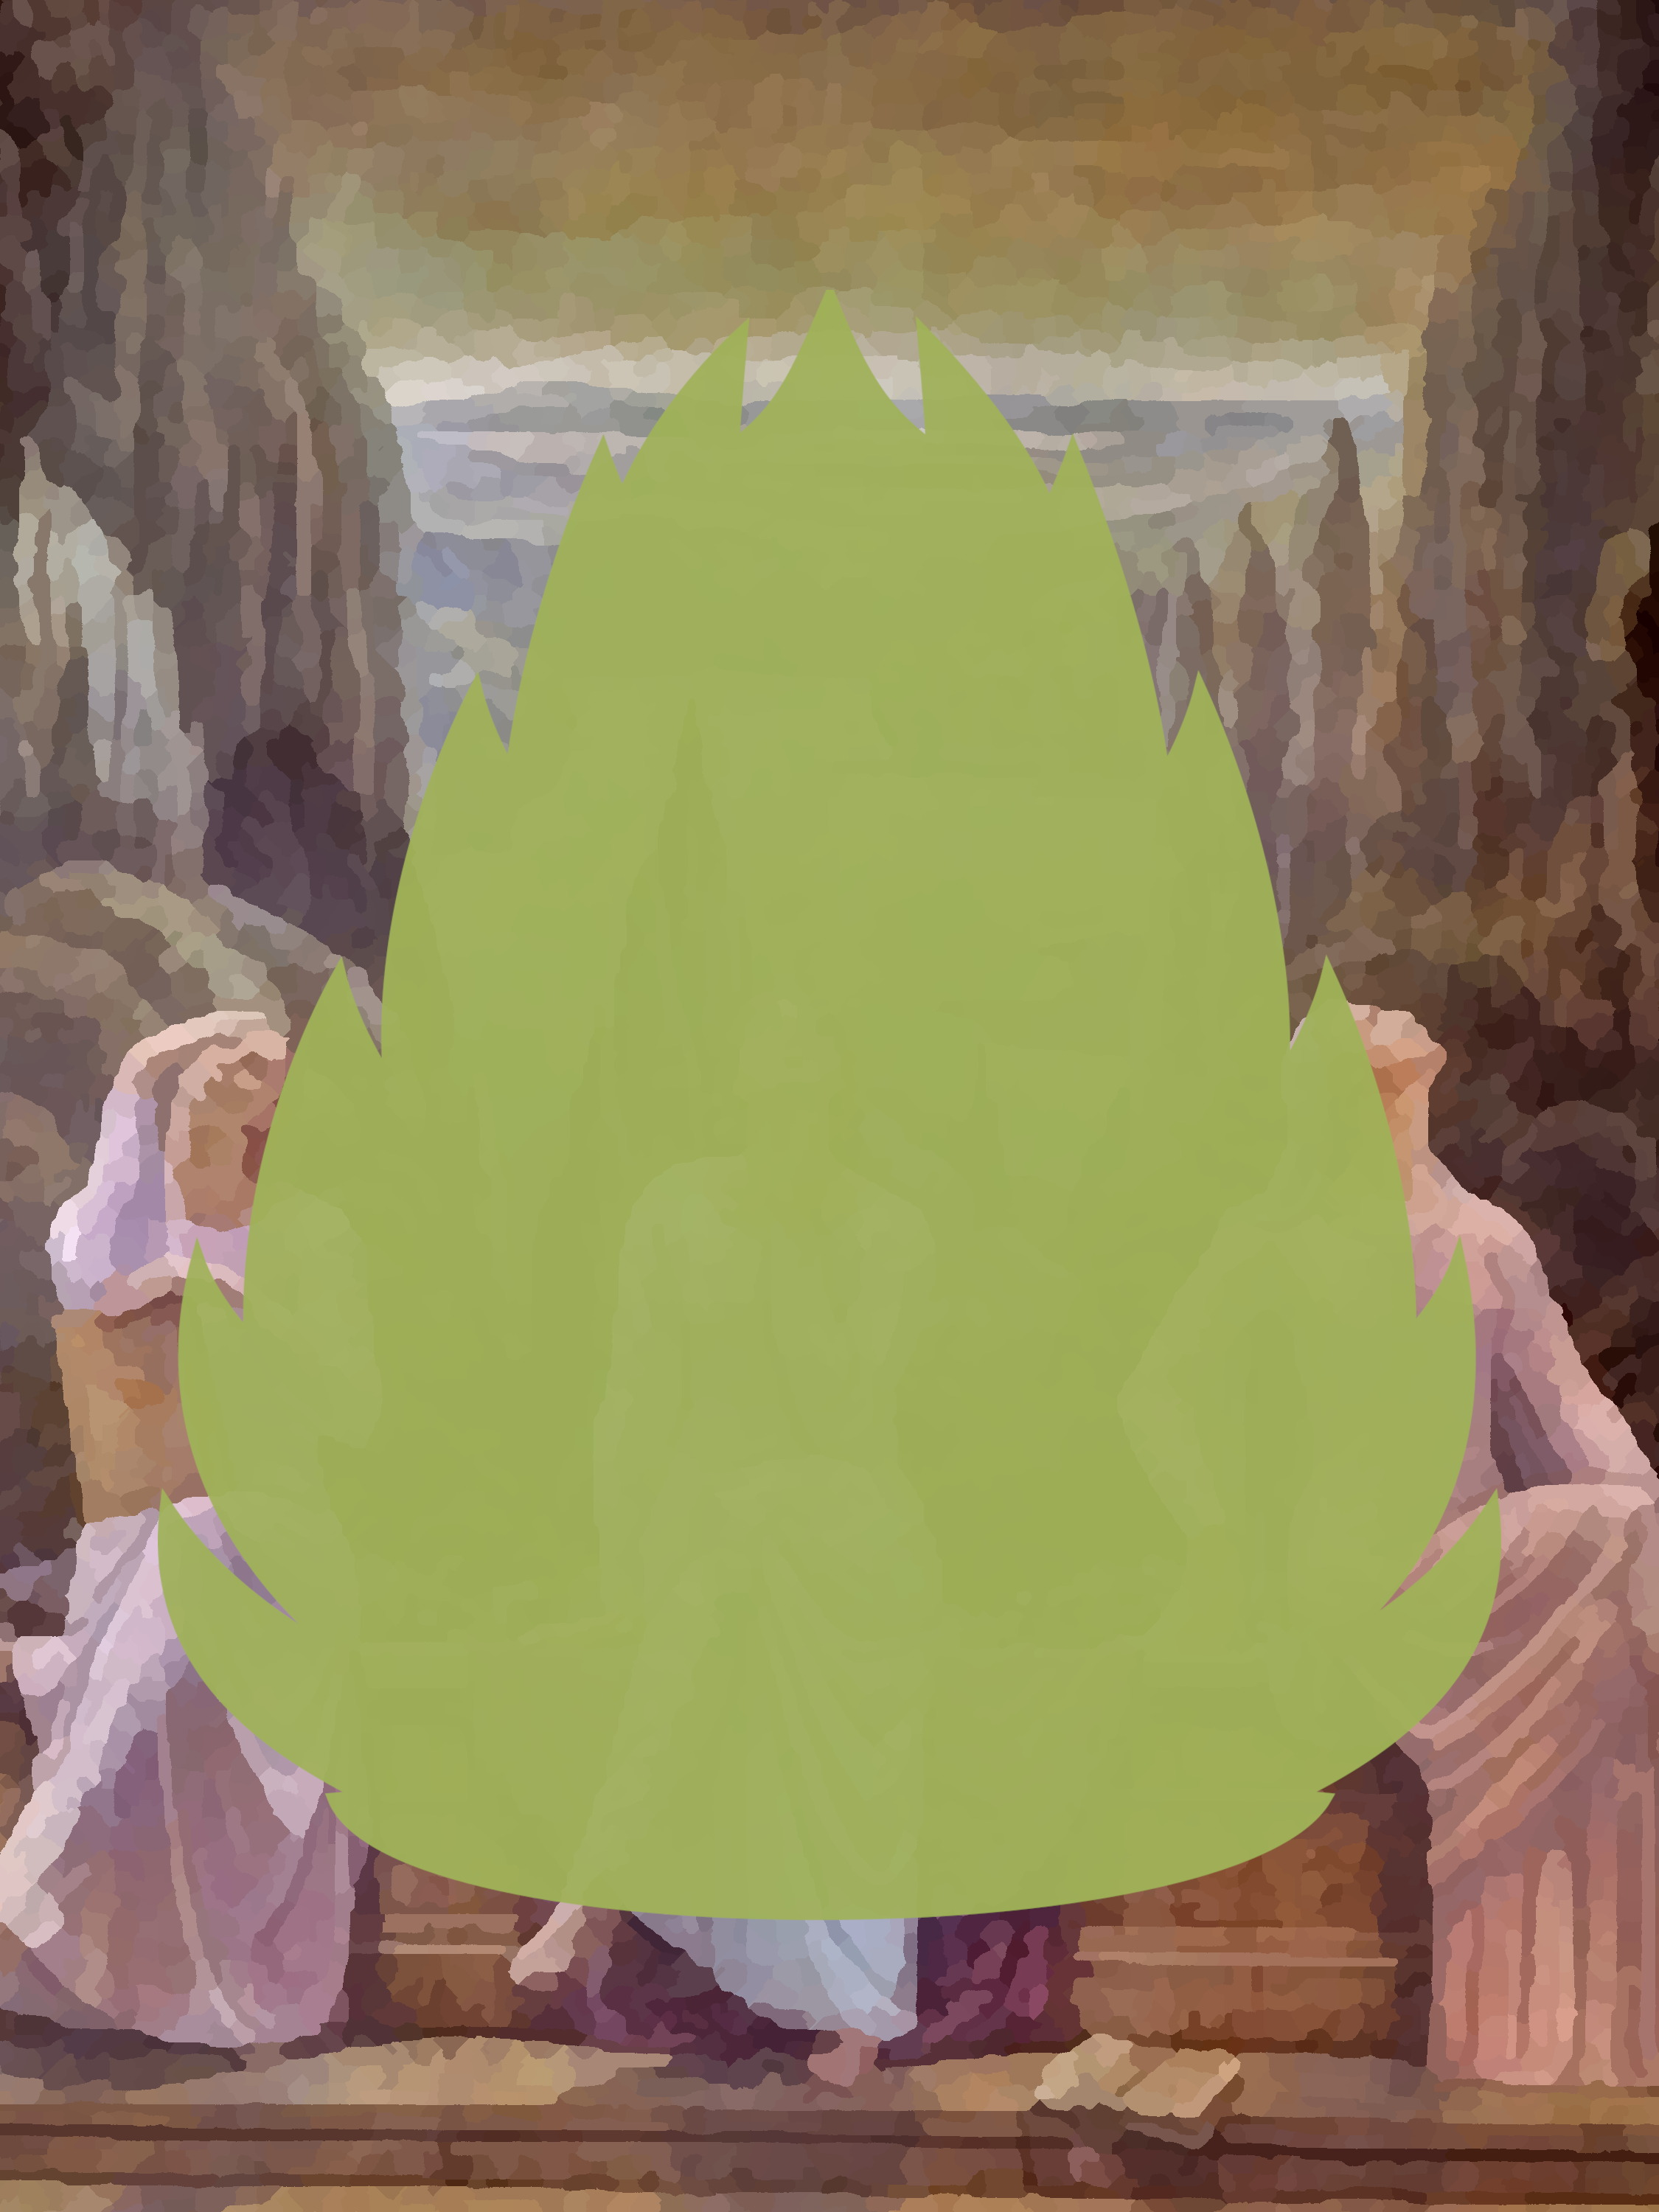
\includegraphics[width=\paperwidth,height=\paperheight]{silence2.jpeg}}

% With XeTeX/LuaTeX, load fontspec after babel to use Unicode
% fonts for Latin script and LGR for Greek:
\ifdefined\luatexversion \usepackage{fontspec}\fi
\ifdefined\XeTeXrevision \usepackage{fontspec}\fi

% "`Lipsiakos" italic font `cbleipzig`:
\newcommand*{\lishape}{\fontencoding{LGR}\fontfamily{cmr}%
		


 \fontshape{li}\selectfont}
\DeclareTextFontCommand{\textli}{\lishape}

\usepackage{booktabs}
\setlength{\emergencystretch}{15pt}
\usepackage{microtype}
\usepackage{fancyhdr}
\begin{document}
\begin{titlepage} % Suppresses headers and footers on the title page
	\centering % Centre everything on the title page
	%\scshape % Use small caps for all text on the title page

	%------------------------------------------------
	%	Title
	%------------------------------------------------
	
	\rule{\textwidth}{1.6pt}\vspace*{-\baselineskip}\vspace*{2pt} % Thick horizontal rule
	\rule{\textwidth}{0.4pt} % Thin horizontal rule
	
	{\scshape\LARGE Hymn to the \\ Goddess of Silence}
	
	\rule{\textwidth}{0.4pt}\vspace*{-\baselineskip}\vspace{3.2pt} % Thin horizontal rule
	\rule{\textwidth}{1.6pt} % Thick horizontal rule

	%------------------------------------------------
	%	Subtitle
	%------------------------------------------------
	
	\vspace{1\baselineskip}
	
	{\scshape By \Large Hildebrand Jacob, \emph{Esq.}} % Subtitle or further description
	





%------------------------------------------------
	%	Cover photo
	%------------------------------------------------
	
	
	%------------------------------------------------
	%	Editor(s)
	%------------------------------------------------


\vspace*{\fill}

	\vspace{1\baselineskip}

	{\footnotesize\scshape Printed for J. Watts at the Printing-Office \\ in \emph{Wild-Court} near \emph{Lincoln's-Inn Fields}.}
	
	{\small\scshape{London, 1734}}
	
	\vspace{0.5\baselineskip} % Whitespace after the title block



\scshape Solar Anamnesis Edition
% Publication year
	
	{\scshape\small CC0 1.0 Universal} % Publisher
\end{titlepage}
\setlength{\parskip}{1mm plus1mm minus1mm}
\setcounter{tocdepth}{3}
\setcounter{secnumdepth}{3}
\clearpage
\begin{center}
Hymn to the Goddess \emph{of Silence}
\end{center}

\bigskip

\begin{quotation}\footnotesize
\hspace*{10mm}ALL Hail! O awful, sage \emph{Divinity!}

\emph{Goddess} of \emph{Silence!} hail! eternal \emph{Pow'r},

Who knowest how the \emph{Universe} was form'd,

How \emph{Nature} first began! for thou wast then,

And startedst at the dread, creating \emph{Voice},

E'en then thou wast, and still thou wilt endure,

When weary'd \emph{Time}, and \emph{Nature} are no more;

At \emph{Desolation} thou again must start,

And the vast \emph{Globe} shall fright thee with its Fall.
\end{quotation}
\begin{quotation}\footnotesize
\hspace*{10mm}Thee, solemn \emph{Being!} venerable \emph{Queen!}

Whose Charms the busy \emph{Vulgar} never know,

Thee the wife \emph{Ancients} justly did revere,

And \emph{Temples} to thy Name devoutly raise.
\end{quotation}
\begin{quotation}\footnotesize
\hspace*{10mm}Thee, \emph{Goddess!} thee, at the still Noon of Night

When all is hush'd, delighted, I adore,

And the pale Moon is witness to thy Rites.
\end{quotation}
\begin{quotation}\footnotesize
\hspace*{10mm}Thee, pleasing \emph{Deity!} the \emph{sacred Nine},

Daughters of \emph{Jove}, the blest \emph{Pierian} Maids

Pursue, and find thee oft in inmost Groves;

On Rocks remote, on shady Banks they meet

Thy kindly Aid, while \emph{Phœbus} ever young,

Immortal \emph{Phœbus} wakes his golden Lyre;

Thy tender Ear can brook the heav'nly Sound:

Thou'rt Friend to \emph{Music}, and harmonious \emph{Verse};

For tho' thou shun'st the noisy, loud \emph{Resorts}

Of restless Man, resounding \emph{Palaces},

The clam'rous \emph{Camp}, the dire, tumultuous \emph{Field},

And oft at the throng'd \emph{Bar} art call'd in vain;

How awful yet o'er crouded \emph{Theatres}

Dost thou preside, when \emph{Johnson's} manly \emph{Scene},

\emph{Shakespear}, or moving \emph{Otway} warms the \emph{Stage?}
\end{quotation}
\begin{quotation}\footnotesize
\hspace*{10mm}O thou, propitious to the tuneful \emph{Quire!}

Where'er thou dost reside, receive my Vows!

Whether in Deserts wild, or Woods remote,

Where yet no Path is made, nor Echoes rude

Frighten the \emph{Dryads} from their lov'd Retreat;

Or whether, lonely, thou delight'st to stray

At \emph{Noontide} on the solitary Plain,

While Flocks, and Herds, and all the rural Rout

Of \emph{Nymphs}, and \emph{Swains} are hid in cooling Shades;

Or is the \emph{Gothic} Temple's gloomy Isle,

The dusky Cloister, or dark Cyprus Grove

Thy lov'd Abode? Or dost thou choose to haunt

(Hard by old \emph{Memphis}, and the fabled \emph{Nile})

The empty Vaults of lofty \emph{Pyramids},

Vain Monuments of ancient \emph{Ægypt}'s Pride?

Or, haply, farther from the World remov'd,

On \emph{Pindus'} Top, or \emph{Atlas'} hoary Crown,

Or some vast Promontory thou dost stand,

Whence scarce the angry \emph{Ocean} is o'erheard,

To lash the hollow, far-resounding Shoar.
\end{quotation}
\begin{quotation}\footnotesize
\hspace*{10mm}Where'er thou'rt found, great \emph{Pow'r}, vouchsafe thy Aid!

Deign visit our Retreat! the sacred \emph{Muse},

The sacred \emph{Muse} with me your Help implores;

Of \emph{War}, and \emph{Sports} by turns we mean to sing,

Of mighty \emph{Heroes}, and of mighty \emph{Love}.

In vain the \emph{God} of \emph{Numbers} doth inspire,

In vain \emph{Apollo}'s Sons attempt to soar

Without thy Influence. Come, Goddess, come!

Bring with thee \emph{Quiet}, \emph{Contemplation},

Poetic \emph{Visions} bright, and \emph{Dreams} sublime,

Such as of old great \emph{Homer} did inspire,

Such as the Gods above themselves may dream,

Still Dreams indeed; but Dreams of mighty \emph{Jove}.

\end{quotation}
\begin{quotation}\footnotesize
\hspace*{10mm}Thus well attended, bless our \emph{Solitude!}

There nothing shall suspend thy gentle Reign,

Save the low Murmur of a distant Stream,

Except by chance sweet \emph{Philomel} complains,

Or \emph{Cloë} tunes her melting Voice, and Lyre.
\end{quotation}
\clearpage
\end{document}
